\section{The \textit{SocVec} Framework}
\label{sec:socvec}
In this section, we first discuss the intuition behind our model, the concept of ``social words'' and our notations. Then, we present the overall workflow of our approach. We finally describe the~\textit{\socvec}~framework in detail.
\subsection{Problem Statement}
We choose (English, Chinese) to be the target language pair throughout this paper for the salient cross-cultural differences between the east and the west\footnote{Nevertheless, the techniques are language independent and 
thus can be utilized for any language pairs so long as 
the necessary resources outlined in \secref{sec:flow} are available.}.
Given an English term $W$ and a Chinese term $U$,
the core research question is 
how to compute a similarity score, $ccsim(W, U)$, to represent the \textit{cross-cultural} \textit{similarities} between them. 

We cannot directly calculate 
the similarity between the monolingual word vectors of $W$ and $U$, 
because they are trained separately and the semantics of dimension
are not aligned.
Thus, the challenge is to devise a way to compute similarities across two different vector spaces while retaining 
their respective cultural characteristics. 
%That is the challenge. 

A very intuitive solution is to firstly translate the Chinese term $U$ to its English 
counterpart $U'$ through a Chinese-English bilingual lexicon, and then regard $ccsim(W, U)$ as 
the (cosine) similarity between $W$ and $U'$ with their monolingual word embeddings.
However, this solution is not promising in some common cases for three reasons: 
\begin{enumerate}[\hspace{0cm}(a)]
	\item if $U$ is an OOV (Out of Vocabulary) term, e.g., a novel slang term, 
	then there is probably no translation $U'$ in bilingual lexicons.
	\item if $W$ and $U$ are names referring to the same named entity, then we have $U' = W$. Therefore, $ccsim(W, U)$ is just the similarity between $W$ and itself, and we cannot capture any cross-cultural differences with this method.
	\item this approach does not explicitly preserve the 
	cultural and social contexts of the terms.
\end{enumerate}

%(i) if $U$ is an OOV (Out of Vocabulary) term, e.g., a slang term, 
%then there is no $U'$ in the bilingual lexicon; 
%%ii) if $U$ is ambiguous and has multiple translations, then the weights
%%of these translated terms are hard to determine;
%(ii) if $W$ and $U$ refer to the same named entity, $U' = W$, 
%then $ccsim(W, U)$ is just the similarity between $W$ and itself, 
%therefore we cannot capture any cross-lingual differences. 
%(iii) this approach does not purposely preserve the 
%cultural and social context of the terms. 
%Therefore, this kind of solutions are not suitable for the two aforementioned 
%tasks, which require the cross-cultural similarities between slang terms 
%and differences between entity names.

To overcome the above problems, our intuition is 
to project both English and Chinese word vectors into a single third space, 
known as \textit{\socvec}, and the projection is supposed to purposely carry 
cultural features of terms.
%Considering the shortcomings of aforementioned transformation-based solutions, we propose to  
%construct a cross-lingual vector space with respect to sociolinguistic features, instead of transforming a space into another one.
%To construct a universal vector space for multilingual usage, we have to specify the meaning of each dimension for each language.
%Meanwhile, the meaning of the dimensions has to be related to opinion, sentiment, cognition and many other psychological processes to help capture the sociolinguistic information.
%Based on these two requirements, we argue that we should build a Bilingual Sociolinguistic Lexicon and extract word representation using the similarities to each translation pair in BSL as a medium.
%


\subsection{Social Words and Our Notations}
%The words people decide to use in their social media messages reflect their beliefs, opinions, and expressions.  
Some research in psychology and sociology~\cite{kitayama2000culture, Gareis_2011} show that culture can be highly related to emotions and opinions people express in their discussions.
%\citet{Tausczik_2009} also suggest that some specific words are much more important than others in analyzing the psychological processes.
As suggested by~\citet{Tausczik_2009}, we thus define the concept of ``\textbf{social word}'' as the words directly reflecting opinion, sentiment, cognition and other human psychological processes\footnote{Example social words in 
	English include \textit{fawn, inept, tremendous, gratitude, terror, terrific, loving, traumatic}, etc. We discuss the sources of such social words in~\secref{sec:prelim}.}, which are important to capturing cultural and social characteristics.
Both \citet{elahi2012examination} and \citet{Garimella2016IdentifyingCD} find such \textit{social words} are 
most effective culture/socio-linguistic features in identifying cross-cultural 
differences. 
%
%\subsection{Notations}

{We use these notations throughout the paper: 
	\textit{CnVec} and \textit{EnVec} denote the Chinese and English word vector space, respectively; 
	\textit{CSV} and \textit{ESV} denote the Chinese and English social word vocab;
	\textit{BL} means Bilingual Lexicon, and \textit{BSL} is short for Bilingual Social Lexicon;
	finally, we use $\bf{E_x}$, $\bf{C_x}$ and $\bf{S_x}$ to denote the word vectors of 
	the word $x$ in \textit{EnVec}, \textit{CnVec} and \textit{\socvec} spaces
	respectively.}


%For convenience, the words in these vocabularies are called
%{\em social words}. 

\begin{figure}[t]
	\centering
	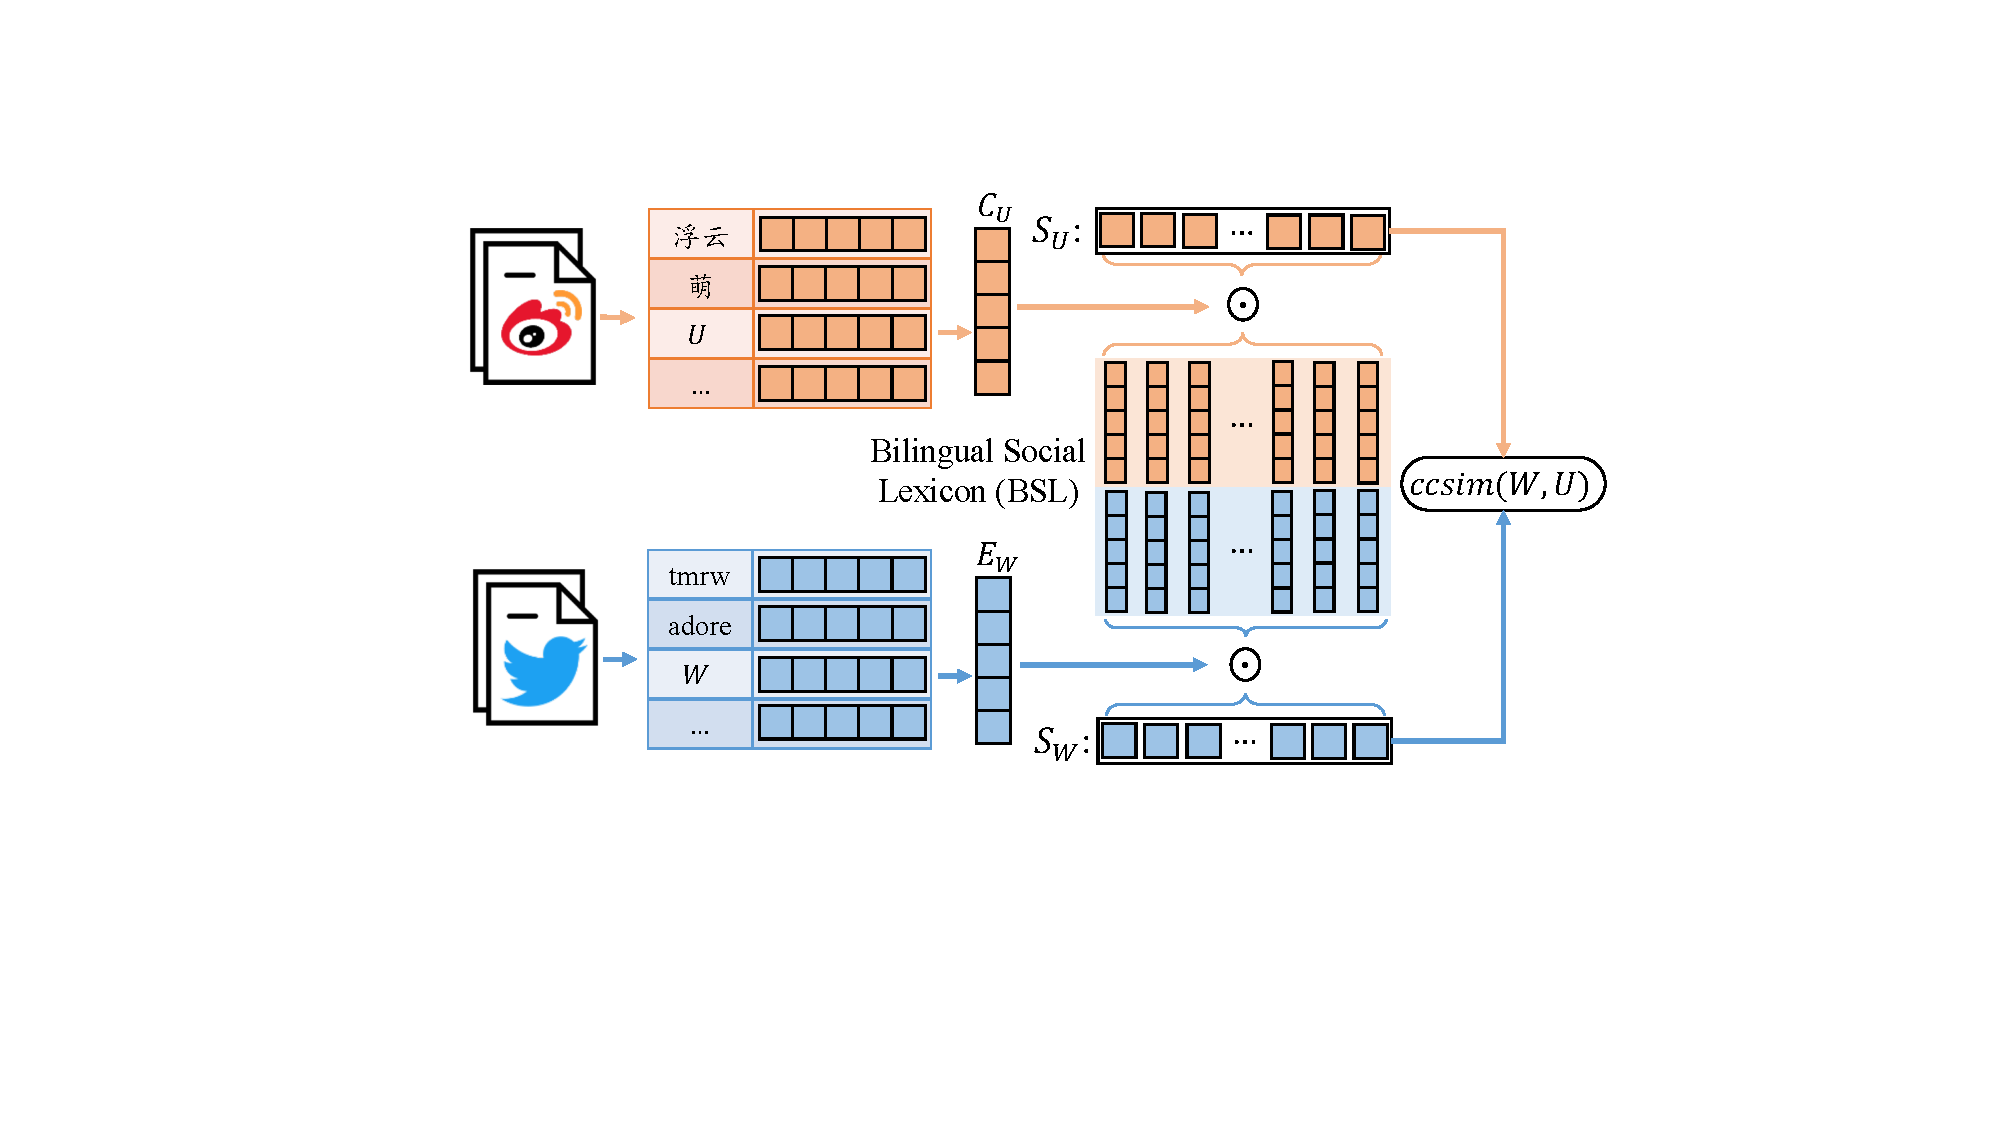
\epsfig{file=figures/framework.pdf, width=1.0\columnwidth}
	\caption{Workflow for computing the cross-cultural similarity between 
		an English word \textit{W} and a Chinese word \textit{U}, denoted by $ccsim(W, U)$}
	%\vspace{-15pt}
	\label{fig:overview}
\end{figure}


%~\footnote{There are open-sourced
%resources for these words as the following sections describe.}
%\BL{maybe use another expression for the social words} 
\subsection{Overall Workflow}
\label{sec:flow}
\figref{fig:overview} shows the workflow of our framework to construct the \textit{\socvec}~and compute $ccsim(W,U)$. 
Our proposed \textit{\socvec}~model attacks the problem with the help of three low-cost external resources: 
(i) an English corpus and a Chinese corpus from social media; (ii) an English-to-Chinese bilingual lexicon (\textit{BL});  
(iii) an English social word vocabulary (\textit{ESV}) and a Chinese one
(\textit{CSV}).

We train English and 
Chinese word embeddings (\textit{EnVec} and \textit{CnVec}) 
on the English and Chinese social media corpus respectively. 
Then, 
we build a \textit{BSL}
from the \textit{CSV}, \textit{ESV} and \textit{BL} (see~\secref{sec:bsl}). 
The \textit{BSL} further maps the previously incompatible \textit{EnVec} and \textit{CnVec} 
into a single common vector space \textit{\socvec},
where two new vectors, $S_W$ for $W$ and $S_U$ for $U$,
are finally comparable.
%
%\subsection{{SocVec} Modeling}
%\label{sec:model}
%In this section, we present the details of SocVec.

\subsection{Building the {BSL}}
\label{sec:bsl}
The process of building the \textit{BSL} is 
illustrated in~\figref{fig:BSL}. 
We first extract our bilingual lexicon (\textit{BL}), where confidence score 
$w_i$ represents the probability distribution on the multiple translations 
for each word. 
Afterwards, we use BL to translate each social word 
in the \textit{ESV} to a set of Chinese words and then filter out all the words that are not in the \textit{CSV}. 
Now, we have a set of Chinese social words for each English social word, which is denoted by a ``translation set''. 
The final step is to generate a Chinese ``pseudo-word'' for each 
English social word using their corresponding translation sets.
{A ``pseudo-word'' can be either a real word that is the most 
representative word in the translation set, or an imaginary word whose 
vector is a certain combination of the vectors of the words in the 
translation set.}

\begin{figure*}[th]
	\centering
	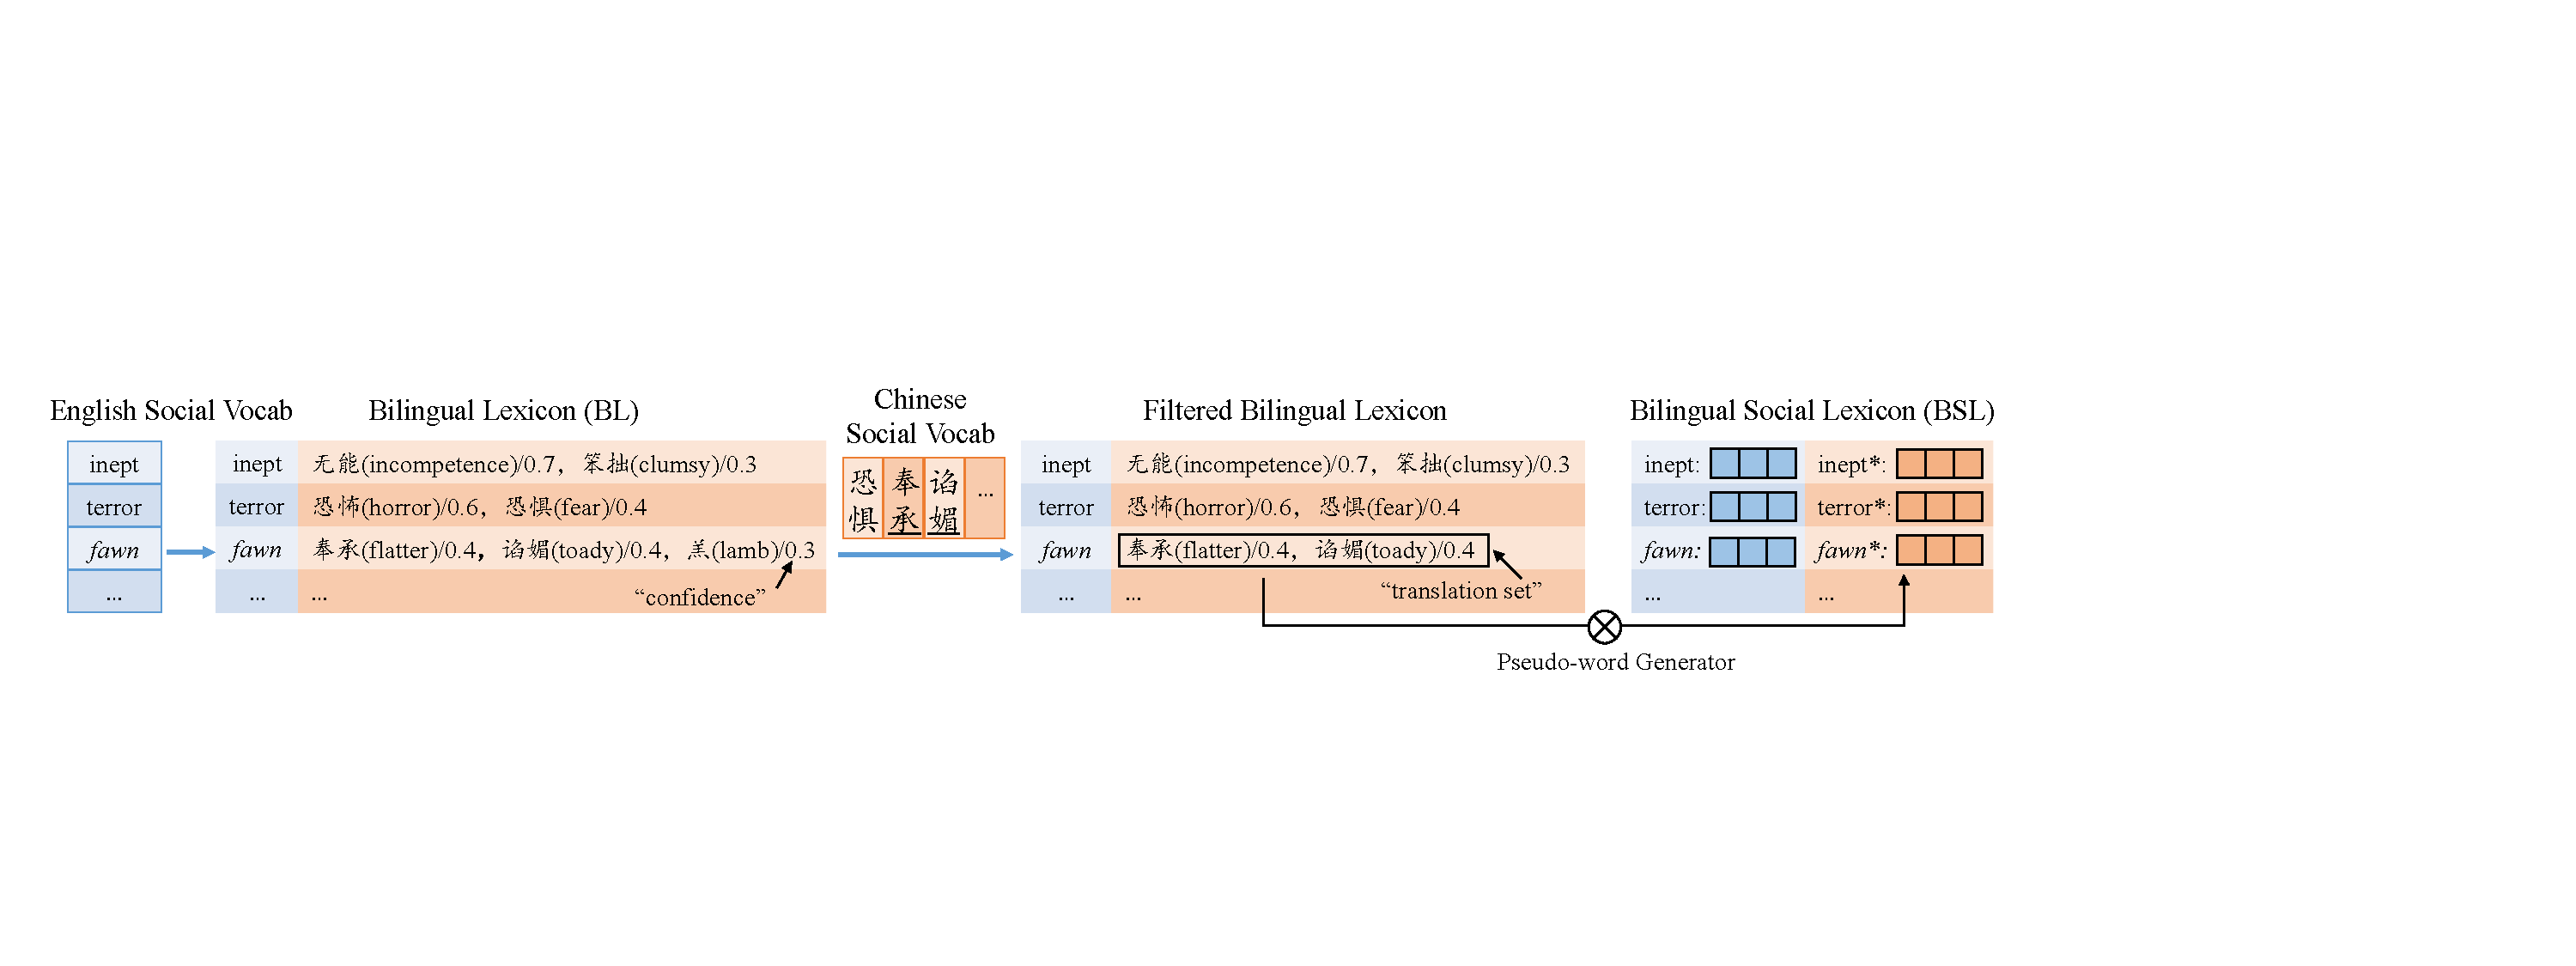
\epsfig{file=figures/bsl.pdf, width=1\textwidth}
	%	\vspace{-15pt}
	\caption{Generating an entry in the BSL for ``\textit{fawn}'' 
		and its pseudo-word ``\textit{fawn}*''}
	\label{fig:BSL}
	%	\vspace{-15pt}
\end{figure*}

For example, in \figref{fig:BSL}, the
English social word ``\textit{fawn}'' has three Chinese translations in the 
bilingual lexicon, but only two of them (underlined) are in the CSV. 
Thus, we only keep these two in the translation set in the filtered bilingual lexicon.
The pseudo-word generator takes the word vectors of the two words (in the black box), namely
奉承 (flatter) and 谄媚 (toady), as input, and generates the pseudo-word 
vector denoted by ``\textit{fawn*}''. {Note that the direction of building \textit{BSL} can also be from Chinese to English, 
	in the same manner. 
	However, we find that the current direction 
		gives better results due to the better translation quality of our \textit{BL} in this direction.}
%\footnote{The reason why we use the direction from English to Chinese  is that English socio-linguistic vocabularies tend to be more accessible and accurate than low-resource languages. The filter is optional for low-resource language which has no socio-linguistic lexicon, if we can afford the inaccuracy.}

Given an English social word, we denote $\mathbf{t_i}$ as the $i^{th}$ Chinese word of its translation set consisting of $N$ social words.
We design four intuitive types of pseudo-word generator as follows, which are tested in the experiments:

\noindent
\textbf{(1) Max.} Maximum of the values in each dimension, assuming dimensionality is $K$:
%\vspace{-10pt}
{\begin{equation*}
	\text{Pseudo}(\mathbf{C_{t_1}},...,\mathbf{C_{t_N}}) = \small \begin{bmatrix}
	max(C_{t_1}^{(1)},...,C_{t_N}^{(1)}) \\
	\vdots   \\
	max(C_{t_1}^{(K)},...,C_{t_N}^{(K)})
	\end{bmatrix}^{\rm T} \\
\end{equation*}}%
\noindent
\textbf{(2) Avg.} Average of the values in every dimension:
{$$\text{Pseudo}(\mathbf{C_{t_1}},...,\mathbf{C_{t_N}})=\frac{1}{N}\sum_i^N\mathbf{C_{t_i}} $$}

\noindent
\textbf{(3) WAvg.} Weighted average value of every dimension 
with respect to the translation confidence:
{$$\text{Pseudo}(\mathbf{C_{t_1}},...,\mathbf{C_{t_N}})=\frac{1}{N}\sum_i^Nw_i \mathbf{C_{t_i}} $$}
\noindent
\textbf{(4) Top.} The most confident translation:
{$$	\text{Pseudo}(\mathbf{C_{t_1}},...,\mathbf{C_{t_N}}) = \mathbf{C_{t_k}}, \text{} k = \argmax_i{w_i} $$}
~~Finally, the \textit{BSL} contains a set of English-Chinese word vector pairs, where each entry represents an English social word and its Chinese pseudo-word based on its ``translation set''.


\subsection{Constructing the {\socvec}~Space}
\label{sec:pg}
%\textbf{Notation Definition.} 

Let $B_i$ denote the English word of the $i^\text{th}$ entry of the \textit{BSL}, and its corresponding Chinese pseudo-word is denoted by $B_i^*$.  
We can project the English word vector $\bf{E_W}$ into the \textit{\socvec} space by 
computing the cosine similarities between $\bf{E_W}$ and each English
word vector in \textit{BSL} as values on~\socvec\ dimensions, effectively constructing a new vector $\bf{S_W}$ of size $L$. 
Similarly, we map a Chinese word vector $\bf{C_U}$ to be a new vector $\bf{S_U}$. 
$\bf{S_W}$ and $\bf{S_U}$ belong to the same vector space \textit{\socvec} 
and are comparable. The following equation illustrates the projection, and how to compute $ccsim$\footnote{{The function $sim$ is a generic similarity function, for which several metrics are considered in experiments.}}.
\begin{align*} 
&ccsim(W,U) := f(\mathbf{E_\text{W}},\mathbf{C_\text U}) \\ 
&=sim\left( 
\small{\begin{bmatrix} 
	cos(\mathbf{E_\text W},\mathbf{E_{ B_1}})\\
	\vdots \\
	cos(\mathbf{E_\text W},\mathbf{E_{B_L}})
	\end{bmatrix}^{\rm T},}
\begin{bmatrix}
cos(\mathbf{C_\text U},\mathbf{C_{B_1^*}})\\
\vdots \\
cos(\mathbf{C_\text U},\mathbf{C_{B_L^*}})
\end{bmatrix}^{\rm T}\right)\\
&=sim(\mathbf{S_\text W},\mathbf{S_\text U})  
\end{align*}
%}%
\normalsize

For example, if $W$ is ``Nagoya'' and $U$ is ``名古屋'', we compute the
cosine similarities between ``Nagoya'' and each English social word in the \textit{BSL} with their monolingual word embeddings in English.
Such similarities compose $\bf{S_{\text{nagoya}}}$. 
Similarly, we compute the cosine similarities
between ``名古屋'' and each Chinese pseudo-word, and compose the social word 
vector $\bf{S_{\text{名古屋}}}$. 

In other words, for each culture/language, the new word vectors like $S_\text W$ are constructed based on the monolingual similarities of each word to the vectors of a set of task-related words (``social words'' in our case). 
This is also a significant part of the novelty of our transformation method. 
%Bridging two cultures and languages by connecting task-related words in different languages is also 

%\scriptsize 
%	\setlength{\abovedisplayskip}{6pt}
%	\setlength{\belowdisplayskip}{\abovedisplayskip}
%	\setlength{\abovedisplayshortskip}{5pt}
%	\setlength{\belowdisplayshortskip}{5pt}
%\noindent where $cos$ denotes the cosine similarity.
%The function $sim$ is a generic similarity function, for which a number of
%metrics will be considered later in experiments.
%
%to project $\mathbf{E_W}$ and $\mathbf{C_U}$ to $\mathbf{S_W}$ and $\mathbf{S_U}$ so that they can be comparable to each other.
%We define the function $f$ to compute cross-lingual similarity between $W$ and $U$ as follows.\footnote{Here $cos$ stands for cosine similarity, } This calculation process is also shown in ~\algref{alg:alg1}. \\
%
%\begin{algorithm}[th]
%	\small
%	\DontPrintSemicolon
%	\caption{Compute cross-lingual similarity between an English word 
%		\textit{W} and a Chinese word \textit{U} } 
%	\label{alg:alg1}
%	\KwIn{ \textit{EnVec}, \textit{CnVec}, $BSL$ with $L$ word pairs} 
%	\KwOut{the cross-lingual similarity $ccsim(W,U)$} 
%	$E_W$ = word vector of $W$ in \textit{EnVec}\\
%	$C_U$ = word vector of $U$ in \textit{CnVec}\\
%	$S_W$ =  zero vector with $L$ dimension \\
%	$S_U$ =  zero vector with $L$ dimension \\
%	%	\Comment*[l]{Project $E_W$ into $S_W$}
%	\For{$1 \le i \le L$}{
%		$B_i$ =  $i^{th}$ English word in \textit{BSL} \\
%		$B_i^*$ = Chinese pseudo-word of $B_i$ \\
%		$S_W[i]$ = $cos(E_W,E_{B_i})$\\
%		$S_U[i]$ = $cos(C_U,C_{B_i^*})$\\
%	} 
%	\Return $ccsim(W,U)$ = $sim(S_W,S_U)$\\
%\end{algorithm}
%\begin{figure}[th!]
%	\centering
%	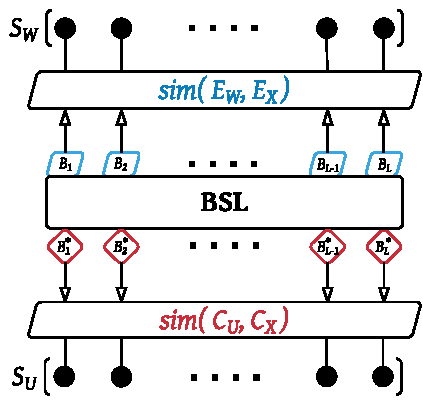
\epsfig{file=figures/SocVec.pdf, width=0.6\columnwidth}
%	\caption{Using \textit{BSL} to project $E_W$ and $C_U$ to $S_W$ and $S_U$.}
%	\label{fig:swsu}
%\end{figure}

%\subsubsection{Parameters Description}
%\label{sec:pd}
%Here, we briefly summarize the main parameters of \textit{SocVec} model:
%\begin{itemize}
%\item Two trained monolingual word embeddings, \textit{EnVec} and \textit{CnVec};  
%\item A bilingual lexicon;
%\item Chinese and English socio-linguistic vocabularies; 
%\item Pseudo-word generator function; 
%\item Option of similarity function $sim$; 
%\end{itemize} 
%We conduct several experiments for testing the these parameters in~\secref{sec:mcdne}.
